\documentclass[11pt]{article}
\usepackage[T1]{fontenc}
\usepackage{lmodern}
\usepackage[margin=1.08in]{geometry}
\usepackage{amsmath,amssymb,amsthm,mathtools}
\usepackage{microtype}
\usepackage{graphicx,booktabs,enumitem}
\usepackage{tikz}
\usetikzlibrary{arrows.meta,calc}
\usepackage[hidelinks]{hyperref}
\hypersetup{pdftitle={The crossing number of complete bipartite graphs},
  pdfauthor={OpenAI},
  pdfsubject={A proof of the Zarankiewicz crossing-number conjecture}}
\pdfinfoomitdate=1
\pdftrailerid{}
\pdfsuppressptexinfo=15
\newcommand{\R}{\mathbb R}
\DeclareMathOperator{\crn}{cr}
\DeclareMathOperator{\rank}{rank}
\DeclareMathOperator{\Span}{span}
\DeclareMathOperator{\diag}{diag}
\newtheorem{theorem}{Theorem}[section]
\newtheorem{lemma}[theorem]{Lemma}
\newtheorem{proposition}[theorem]{Proposition}
\newtheorem{corollary}[theorem]{Corollary}
\theoremstyle{remark}
\newtheorem{remark}[theorem]{Remark}
\numberwithin{equation}{section}
\setlist[itemize]{topsep=4pt,itemsep=2pt}
\setlist[enumerate]{topsep=4pt,itemsep=2pt}
\setlength{\emergencystretch}{1.5em}
\title{The crossing number of complete bipartite graphs}
\author{OpenAI}
\date{September 23, 2026}

\begin{document}
\maketitle
\begin{abstract}
We prove the Zarankiewicz crossing-number conjecture, resolving Tur\'an's
brickyard problem. For all positive integers $m,n$, the ordinary crossing
number of the complete bipartite graph $K_{m,n}$ is
\[
 \left\lfloor\frac m2\right\rfloor
 \left\lfloor\frac{m-1}{2}\right\rfloor
 \left\lfloor\frac n2\right\rfloor
 \left\lfloor\frac{n-1}{2}\right\rfloor.
\]
\end{abstract}

\section{Introduction}
\label{sec:introduction}

For a finite graph $G$, a plane drawing places its vertices at distinct
points and represents each edge by a simple continuous arc whose interior
avoids the vertices. A meeting of two edge interiors is a proper crossing
if some open neighborhood of the point has a homeomorphism onto an open
disk taking the point to its center and the two local edge traces onto its
horizontal and vertical diameters. We require that edge interiors meet at
finitely many proper crossings, with no triple crossings, tangencies, or
common subarcs.
The number $c(D)$ of a drawing $D$ counts crossing points: if two edges
cross several times, each crossing is counted.
The ordinary crossing number is
\[
  \crn(G)=\min_D c(D).
\]
There are no restrictions on vertex positions or on edge routes.

Let $K_{m,n}$ be the complete bipartite graph with vertex classes
$\{a_1,\ldots,a_m\}$ and $\{b_1,\ldots,b_n\}$. Put
\begin{equation}
\label{eq:dr}
 d_r=\left\lfloor\frac r2\right\rfloor
     \left\lfloor\frac{r-1}{2}\right\rfloor
 =\binom{\lfloor r/2\rfloor}{2}
  +\binom{\lceil r/2\rceil}{2}.
\end{equation}
\begin{theorem}
\label{thm:main}
For all positive integers $m,n$,
\[
 \crn(K_{m,n})=d_m d_n.
\]
\end{theorem}

The distinction between crossing points, crossing pairs, and parity-based
crossing counts is important; we use the ordinary point-count convention
throughout~\cite{PachToth2000,FulekEtAl2012}.

Tur\'an described the problem's origin in rail connections between kilns
and storage yards at a brick factory near Budapest in
1944~\cite[pp.~8--9]{Turan1977}.
Zarankiewicz supplied the balanced-axis construction, but the published
argument for its optimality contained a gap
\cite{Zarankiewicz1955,Turan1977,ErdosGuy1973}.
Kleitman established the exact formula when one vertex class has at
most six vertices~\cite{Kleitman1970}.
His permutation argument already used the local cyclic orders of incident
edges to bound crossings between two stars
\cite[Section~8, equation~(17)]{Kleitman1970}.
Woodall developed this approach through cyclic-order graphs and verified the cases
$K_{7,7}$ and $K_{7,9}$ by computation~\cite{Woodall1993}.
The rotation constraints later supported semidefinite lower bounds
\cite{deKlerkEtAl2006,deKlerkPasechnikSchrijver2007}, refined for fixed
part sizes by Brosch and Polak~\cite{BroschPolak2024}.
For balanced graphs, Balogh, Lidick\'y, Norin, Pfender, Salazar, and
Spiro obtained
\[
 \operatorname{cr}(K_{n,n})\ge0.9118\,d_n^2+o(n^4)
\]
using Razborov's flag-algebra method~\cite{Razborov2007,BaloghEtAl2023}.
Hebbar and Mangam have also published claims of both the complete-graph
and complete-bipartite formulas~\cite{HebbarMangam2018}.
Theorem~\ref{thm:main} resolves the Zarankiewicz crossing-number
conjecture positively through the self-contained argument below.

Tutte developed an algebraic approach to crossing
numbers~\cite{Tutte1970}. Our proof combines signed intersections of edge
interiors with a contribution determined by the incident-edge order at a
common endpoint. The resulting cycle pairing separates the topological
information from the algebraic estimates.

The proof separates the geometry of a drawing from two linear-algebraic
statements. In Section~\ref{sec:subspaces}, we prove that subspaces
$U_i,V_i$ of an $N$-dimensional
real vector space satisfying $U_i\cap V_i=0$ obey
\begin{equation}
\label{eq:intro-subspaces}
 \sum_{i,j=1}^m\dim(U_i\cap V_j)
 \le \left\lfloor\frac{m^2}{4}\right\rfloor N.
\end{equation}
The argument uses interpolation with subspace constraints at finitely many
nodes and counts the zeros of polynomial minors. Related determinant
multiplicity arguments control sums of intersection dimensions in the
theory of subspace designs~\cite{GuruswamiKopparty2016}.
Here the degree filtration is adapted to arbitrary subspaces $U_i$;
diagonal disjointness bounds the rank at the interpolation nodes.
Applied to graphs of linear maps, the resulting inequality gives a lower
bound on the sum of the ranks of differences $X_i-Y_j$ of square
matrices, provided every diagonal difference $X_i-Y_i$ is invertible.
Both formulations are independent of graph drawings.

In Section~\ref{sec:detector}, for odd $n=2s+1\ge3$, we construct a linear map from $n$-by-$n$
matrices to $s^2$-by-$s^2$ matrices. It annihilates row-plus-column terms
and diagonal entries and sends each individual matrix entry to a matrix of
rank at most one. For a linear order $\prec$ on $\{1,\ldots,n\}$, let
$S_\prec$ be half its comparison-sign matrix: its $(p,q)$ entry is
$\tfrac12$ if $p\prec q$, $-\tfrac12$ if $q\prec p$, and $0$ if $p=q$.
The map sends every $S_\prec$ to an invertible matrix.
The construction uses the classical barycentric weights for Lagrange interpolation
\cite[Sections~2--3]{BerrutTrefethen2004} and bivariate monomial evaluations;
its invertibility reduces to interpolation on two complementary triangles
of an evaluation grid.

To connect these statements, normalize a minimum drawing $D$ so its
edges are polygonal and adjacent edges do not cross. Orient edges from
the first vertex class to the second. At each vertex, read the counterclockwise
spoke order from a chosen gap. Form a matrix $J$ indexed by these
edges. Its entry for two distinct edges is their signed crossing count,
plus half their comparison sign in the incident order if they share an
endpoint; diagonal entries are zero. The block $J^{ik}$
compares the edges incident with $a_i$ to those incident with $a_k$.
The vanishing of algebraic intersections of closed plane curves makes
these blocks additive modulo row-plus-column terms
(Section~\ref{sec:intersections}).
Applying the linear map produces
the family $X_i-Y_j$: diagonal blocks have full rank, and off-diagonal
ranks are bounded by the corresponding crossing counts.
Corollary~\ref{cor:rank-sum} bounds the ordered sum of off-diagonal
ranks below by $2d_m d_n$. The corresponding sum of crossing counts
counts each crossing twice, so the rank sum is at most $2c(D)$.
This gives $c(D)\ge d_m d_n$.
Section~\ref{sec:formula} completes the proof: deleting vertices gives
the even case, and the classical balanced-axis drawing gives the
matching upper bound.

Every ingredient of the lower-bound argument is proved below.
For completeness, Appendix~\ref{sec:normalization} supplies the drawing
reductions for the continuous-arc definition used here.

\section{A subspace intersection inequality}
\label{sec:subspaces}

The algebraic estimate behind the lower bound concerns arbitrary pairs of
subspaces.  The only hypothesis is that each subspace is disjoint from its
designated partner. Polynomial determinants have also been used to
control sums of intersection dimensions in subspace designs
\cite{GuruswamiKopparty2016}. Here the degree filtration is adapted
to the arbitrary family $U_i$, and all details are proved below.

\begin{lemma}[Subspace intersection bound]
\label{lem:subspace}
Let $W$ be a real vector space of dimension $N$, and let
$U_1,\ldots,U_m,V_1,\ldots,V_m$ be subspaces of $W$, where $m\geq1$.
If $U_i\cap V_i=\{0\}$ for every $i$, then
\begin{equation}
\label{eq:subspace-bound}
  \sum_{i,j=1}^{m}\dim(U_i\cap V_j)
  \leq \left\lfloor\frac{m^2}{4}\right\rfloor N.
\end{equation}
\end{lemma}

\begin{proof}
We encode the subspaces by polynomial evaluation constraints.  Evaluating
away from the constraint nodes gives a filtration of evaluation spaces.
At each node, disjointness bounds the evaluated rank.  The resulting
rank deficiency gives a lower bound on a polynomial minor's vanishing
order.  Comparing these orders with the minor's degree, then summing
over the filtration, will give the bound.

Choose distinct real numbers $t_1,\ldots,t_m$.  For a subspace $Z\subseteq W$
and an integer $h\geq0$, define
\[
  \mathcal P_h(Z)=
  \{P\in Z[\xi]:\deg P\leq h,\ P(t_i)\in U_i\text{ for every }i\},
  \qquad \mathcal P_{-1}(Z)=\{0\}.
\]
Here $Z[\xi]$ denotes polynomials whose coefficients belong to $Z$.
Write $E_h(Z;t)=\{P(t):P\in\mathcal P_h(Z)\}$ and put
\[
  k_h(Z)=\dim\mathcal P_h(Z)-\dim\mathcal P_{h-1}(Z),
  \qquad k_{-1}(Z)=0.
\]

\emph{Evaluation away from the nodes.}
For $t\notin\{t_1,\ldots,t_m\}$, the kernel of evaluation at $t$ is
\[
  \ker\bigl(\mathcal P_h(Z)\longrightarrow Z,\ P\longmapsto P(t)\bigr)
  =(\xi-t)\mathcal P_{h-1}(Z).
\]
Indeed, division by $\xi-t$ preserves the coefficient space $Z$, and it
preserves each constraint at $t_i$ because $t_i-t\ne0$.  The converse
inclusion follows by multiplication.  Therefore
\begin{equation}
\label{eq:filtration-evaluation}
  \dim E_h(Z;t)=k_h(Z)
  \qquad(t\notin\{t_1,\ldots,t_m\}).
\end{equation}
Also, evaluation at all $m$ nodes is an isomorphism
\[
  \mathcal P_{m-1}(Z)\longrightarrow
  \bigoplus_{i=1}^{m}(U_i\cap Z).
\]
Its inverse sends $(z_1,\ldots,z_m)$ to the polynomial
$\sum_i L_i(\xi)z_i$, where
$L_i(\xi)=\prod_{k\ne i}(\xi-t_k)/(t_i-t_k)$.
Uniqueness follows because a scalar polynomial of degree at most $m-1$
with $m$ distinct roots vanishes, applied in coordinates of $Z$.
Consequently
\begin{equation}
\label{eq:filtration-sum}
  \sum_{h=0}^{m-1}k_h(Z)
  =\dim\mathcal P_{m-1}(Z)
  =\sum_{i=1}^{m}\dim(U_i\cap Z).
\end{equation}

\emph{Polynomial minors of controlled degree.}
Fix $t_*$ outside the nodes.  The spaces $E_h(W;t_*)$ are nested, so
\[
  \ell_h=k_h(W)-k_{h-1}(W)\geq0
  \qquad(0\leq h\leq m-1).
\]
At stage $h$, choose $\ell_h$ polynomials from $\mathcal P_h(W)$ whose
values at $t_*$ extend the previously chosen values to a basis of
$E_h(W;t_*)$.  In fixed coordinates of $W$, let $M_h(\xi)$ be the matrix
of all polynomial columns chosen through stage $h$.  It has
$r_h=k_h(W)$ columns, independent at $t_*$, and hence has an $r_h$-row
square minor $\Delta_h(\xi)$ with $\Delta_h(t_*)\ne0$.  Each column
introduced at stage $e$ has degree at most $e$.  Expanding the determinant
thus gives
\begin{equation}
\label{eq:minor-degree}
  \deg\Delta_h\leq\sum_{e=0}^{h}e\ell_e.
\end{equation}
If $r_h=0$, use the empty determinant $\Delta_h=1$.

\emph{Rank loss at the nodes.}
For each $j$ we claim that
\begin{equation}
\label{eq:node-rank}
  \dim E_h(W;t_j)\leq k_h(W)-k_h(V_j).
\end{equation}
Let $\pi_j:W\longrightarrow W/V_j$ be the quotient map.  At every
non-node $t$, the kernel of $\pi_j$ on $E_h(W;t)$ contains
$E_h(V_j;t)$.  Equation~\eqref{eq:filtration-evaluation} gives
\[
  \dim\pi_j(E_h(W;t))\leq k_h(W)-k_h(V_j).
\]
To pass to $t_j$, take a fixed basis of the polynomial space
$\mathcal P_h(W)$, evaluate its members at the variable $\xi$, and project
their columns by $\pi_j$.  In fixed coordinates this is a polynomial
matrix.  Every minor larger than the displayed rank bound vanishes at
every non-node, an infinite set, and so is the zero polynomial.  Its rank
at $t_j$ obeys the same bound.  But $E_h(W;t_j)\subseteq U_j$, and $\pi_j$
is injective on $U_j$ because $U_j\cap V_j=\{0\}$.  This proves
\eqref{eq:node-rank}.

The chosen columns of $M_h(t_j)$ lie in $E_h(W;t_j)$, and restricting
to the rows of a minor cannot increase rank.
The square submatrix defining $\Delta_h$ therefore has rank deficiency
at least $k_h(V_j)$ at $t_j$.  A square polynomial matrix with deficiency
at least $q$ at $t_j$ has determinant divisible by $(\xi-t_j)^q$:
choose $q$ independent vectors in its kernel at $t_j$, extend them to
a constant invertible column change, and observe that the corresponding
$q$ transformed columns vanish at $t_j$.  Each contributes the factor
$\xi-t_j$, while the column change rescales the determinant by a nonzero
constant.  Applying this observation separately at the distinct nodes
shows that
\[
  \prod_{j=1}^{m}(\xi-t_j)^{k_h(V_j)}\quad\text{divides }\Delta_h(\xi).
\]
For $r_h=0$, all $k_h(V_j)$ are zero by
\eqref{eq:filtration-evaluation}, so this assertion also holds for the
empty determinant.  Since $\Delta_h$ is not the zero polynomial,
\eqref{eq:minor-degree} now yields
\begin{equation}
\label{eq:multiplicity-budget}
  \sum_{j=1}^{m}k_h(V_j)\leq\sum_{e=0}^{h}e\ell_e.
\end{equation}

\emph{Summing the degree bounds.}
Sum \eqref{eq:multiplicity-budget} over $h=0,\ldots,m-1$ and apply
\eqref{eq:filtration-sum} with $Z=V_j$.  The result is
\begin{align*}
  \sum_{i,j=1}^{m}\dim(U_i\cap V_j)
  &\leq\sum_{h=0}^{m-1}\sum_{e=0}^{h}e\ell_e
   =\sum_{e=0}^{m-1}e(m-e)\ell_e\\
  &\leq\left\lfloor\frac{m^2}{4}\right\rfloor
           \sum_{e=0}^{m-1}\ell_e
   \leq\left\lfloor\frac{m^2}{4}\right\rfloor N.
\end{align*}
The last step uses
$\sum_e\ell_e=k_{m-1}(W)=\dim E_{m-1}(W;t_*)\leq N$.
\end{proof}

\begin{remark}
The constant in Lemma~\ref{lem:subspace} is sharp.  Write $W=P\oplus Q$
and divide the indices into groups of sizes $a=\lfloor m/2\rfloor$ and
$b=\lceil m/2\rceil$.  Set $(U_i,V_i)=(P,Q)$ in the first group and
$(U_i,V_i)=(Q,P)$ in the second.  Only pairs from different groups
contribute, and their total is $ab(\dim P+\dim Q)=\lfloor m^2/4\rfloor N$.
\end{remark}

The form needed for crossing counts follows by taking graphs of linear
maps.  Their intersections identify with kernels of matrix differences, so the
upper bound on intersection dimensions becomes a lower bound on ranks.

\begin{corollary}[Rank sum for differences]
\label{cor:rank-sum}
Let $X_1,\ldots,X_m,Y_1,\ldots,Y_m$ be real $d\times d$ matrices.
If $X_i-Y_i$ is invertible for every $i$, then
\begin{equation}
\label{eq:rank-sum}
  \sum_{\substack{1\leq i,j\leq m\\i\ne j}}
       \rank(X_i-Y_j)\geq2d_m d,
  \qquad
  d_m=\left\lfloor\frac m2\right\rfloor
      \left\lfloor\frac{m-1}{2}\right\rfloor.
\end{equation}
The sum is over ordered pairs of distinct indices.
\end{corollary}

\begin{proof}
In $W=\R^d\oplus\R^d$, let
\[
  U_i=\{(v,X_iv):v\in\R^d\},\qquad
  V_j=\{(v,Y_jv):v\in\R^d\}.
\]
The map $v\mapsto(v,X_iv)$ identifies $\ker(X_i-Y_j)$ with
$U_i\cap V_j$.  Thus
\[
  \dim(U_i\cap V_j)=d-\rank(X_i-Y_j),
  \qquad U_i\cap V_i=\{0\}.
\]
Lemma~\ref{lem:subspace}, with $N=2d$, gives
\[
  \sum_{i,j=1}^{m}\rank(X_i-Y_j)
  \geq\left(m^2-2\left\lfloor\frac{m^2}{4}\right\rfloor\right)d.
\]
The $m$ diagonal terms each equal $d$.  Removing them gives
\eqref{eq:rank-sum}, because
\[
  m^2-m-2\left\lfloor\frac{m^2}{4}\right\rfloor
  =\begin{cases}
      2r(r-1),&m=2r,\\
      2r^2,&m=2r+1,
    \end{cases}
  =2d_m.
\]
\end{proof}

\section{Signed intersections and cycle relations}
\label{sec:intersections}

Signed intersections of cycles impose relations on the crossing data
between stars. We derive the block relation needed to apply the
rank-sum inequality.

Fix a minimum drawing $D$ of $K_{m,n}$.  By
Lemma~\ref{lem:normalization}, proved in Appendix~\ref{sec:normalization},
we may take its edges to be polygonal, straight in a neighborhood of
every crossing and vertex, with no crossings between edges having a
common endpoint.  Independent edges may still cross several times.
Orient the edge $ip$ from $a_i$ to $b_p$.

For oriented edges $e,f$, let $I(e,f)$ be the sum of the signs of their
interior crossings.  A crossing is positive when the ordered directions
of $e$ and $f$ give the positive orientation of the plane.  Set
$I(e,e)=0$.
At a vertex $v$, choose a gap between consecutive outward spokes and list
the incident edges counterclockwise from that gap.  Define
\[
 T_v(e,f)=
 \begin{cases}
  1,&e\text{ precedes }f,\\
  -1,&f\text{ precedes }e,\\
  0,&e=f,
 \end{cases}
 \qquad
 \sigma_{ve}=
 \begin{cases}
  1,&e\text{ is oriented out of }v,\\
  -1,&e\text{ is oriented into }v.
 \end{cases}
\]
The matrix indexed by the edges that we use is
\begin{equation}
 \label{eq:signed-J}
 J(e,f)=I(e,f)+\frac12
 \sum_{\substack{v\text{ an endpoint}\\\text{of both }e,f}}
 \sigma_{ve}\sigma_{vf}T_v(e,f),
 \qquad J^{ik}(p,q)=J(ip,kq).
\end{equation}
Thus $J^{ik}$ is an $n\times n$ block.  The half-order term records the
local contribution of a common endpoint to an intersection of cycles.
The next lemma identifies precisely that contribution.

\begin{lemma}[Cycle pairing]
\label{lem:cycle-pairing}
Let $z,y\in\R^{E(K_{m,n})}$ be the signed edge vectors of two oriented
simple graph cycles: an entry is $1$ or $-1$ according as the traversal
agrees or disagrees with the fixed edge orientation, and is $0$ on an
unused edge.  Then
\begin{equation}
 \label{eq:cycle-pairing}
 z^{\mathsf T}Jy=0.
\end{equation}
The cycles may share vertices and edges, and may traverse a shared edge
in opposite directions.
\end{lemma}

\begin{proof}
We first establish the local formula that explains the factor $1/2$.
Let $C$ and $E$ be oriented chords of a round disk, with four distinct
boundary endpoints.  Give each chord's start coefficient $-1$ and its
end coefficient $+1$; write these coefficients as $\epsilon_C(u)$ and
$\epsilon_E(w)$.  For a cut in the boundary away from the endpoints,
let $T(u,w)$ be $1$ if $u$ precedes $w$ counterclockwise from the cut,
and $-1$ otherwise.  Their signed intersection is
\begin{equation}
 \label{eq:chord-formula}
 I(C,E)=\frac12\sum_{u\in\partial C}\sum_{w\in\partial E}
       \epsilon_C(u)\epsilon_E(w)T(u,w).
\end{equation}
Moving the cut past one endpoint changes the right-hand side by a
multiple of the sum of the other chord's endpoint coefficients, which
is zero.  We may therefore cut just before the start of $C$.
The right-hand side then becomes
\[
 -\sum_{\substack{w\text{ on the open counterclockwise arc}\\
                 \text{from the start to the end of }C}}
        \epsilon_E(w).
\]
That boundary arc is on the right of the directed chord $C$.  The sum
is zero for nonalternating endpoints; for alternating endpoints it is
$+1$ when $E$ runs from right to left across $C$, and $-1$ in the reverse
case.  These are exactly the signed intersection values.

Figure~\ref{fig:chord-pairing} illustrates the local signs and the
averaging at a shared spoke used below.
\begin{figure}[tb]
\centering
\begin{minipage}[t]{.47\textwidth}
\centering
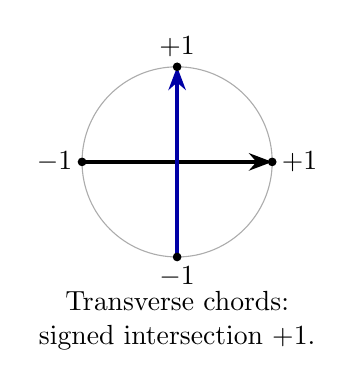
\begin{tikzpicture}[scale=1.05,>=Stealth]
  \draw[gray!65] (0,0) circle (1.15);
  \draw[->,very thick] (-1.15,0)--(1.15,0);
  \draw[->,very thick,blue!65!black] (0,-1.15)--(0,1.15);
  \foreach \x/\y in {-1.15/0,1.15/0,0/-1.15,0/1.15}
    \fill (\x,\y) circle (1.5pt);
  \node[left] at (-1.15,0) {$-1$};
  \node[right] at (1.15,0) {$+1$};
  \node[below] at (0,-1.15) {$-1$};
  \node[above] at (0,1.15) {$+1$};
  \node[align=center] at (0,-1.92) {Transverse chords:\\signed intersection $+1$.};
\end{tikzpicture}
\end{minipage}\hfill
\begin{minipage}[t]{.50\textwidth}
\centering
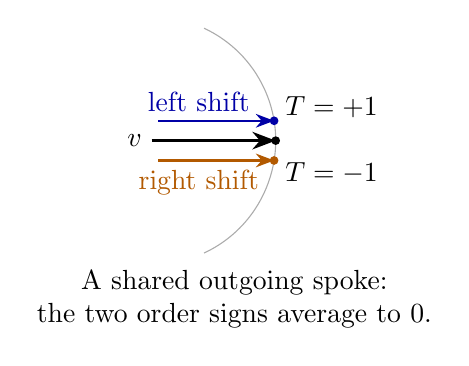
\begin{tikzpicture}[scale=1.05,>=Stealth]
  \draw[gray!65] (-65:1.5) arc[start angle=-65,end angle=65,radius=1.5];
  \draw[->,very thick] (0,0)--(1.5,0);
  \draw[->,thick,blue!65!black] (.08,.24)--(1.4807,.24);
  \draw[->,thick,orange!70!black] (.08,-.24)--(1.4807,-.24);
  \fill (1.5,0) circle (1.5pt);
  \fill[blue!65!black] (1.4807,.24) circle (1.5pt);
  \fill[orange!70!black] (1.4807,-.24) circle (1.5pt);
  \node[left] at (0,0) {$v$};
  \node[above,blue!65!black] at (.57,.24) {left shift};
  \node[below,orange!70!black] at (.57,-.24) {right shift};
  \node[right] at (1.50,.40) {$T=+1$};
  \node[right] at (1.50,-.40) {$T=-1$};
  \node[align=center] at (1,-1.92) {A shared outgoing spoke:\\the two order signs average to $0$.};
\end{tikzpicture}
\end{minipage}
\caption{The local terms in the signed-intersection identity.
The coefficient of a chord's start is $-1$ and that of its end is $+1$.
For a common spoke, the opposite displacements are considered in separate
drawings; the chosen cut is away from all three nearby endpoints.}
\label{fig:chord-pairing}
\end{figure}


Choose small pairwise disjoint round vertex disks meeting the drawing
only in its straight spokes.  Replace the passage of the first cycle
through each of its vertex disks by the chord joining its incoming
and outgoing boundary points.  Outside these disks, keep its original
edge tracks.  This gives a closed polygonal walk $\gamma$; its drawing
may have self-intersections.

For the second cycle construct two closed polygonal walks
$\eta_+$ and $\eta_-$ by shifting its edge tracks a small distance to
the left and to the right, respectively, relative to the \emph{fixed
graph-edge orientation}.  In each vertex disk join the shifted
boundary endpoints by a chord.  Here is an explicit construction of
the tracks outside the vertex disks.  Place further pairwise disjoint
small disks at crossings and nonstraight bends, each meeting only the
straight pieces incident with its center.  Shift each straight stretch
between disks parallel to itself.  In a crossing disk continue along
the shifted line: it avoids its own original line and meets the other
original line once, with the same crossing sign.  In a bend disk the
two shifted ends lie in the same component of the disk minus the
original bent arc, and can be joined there by a polygonal arc.  Indeed,
for the left shift, the incoming boundary ray moves clockwise and the
outgoing ray counterclockwise; both displaced ends are in the sector
on the left of the oriented bend.  The right shift uses the other
sector.  All remaining distinct truncated straight stretches are
compact and disjoint, so sufficiently small shifts introduce no
additional intersections.  Finiteness permits one choice of shift
size for the entire construction. At vertex-circle seams the two walks'
boundary endpoints are distinct and chord interiors lie in the open disk;
at crossing disks the intended intersections remain strictly interior.
Together with the avoidance inside bend disks, this excludes contacts
at seams and corners.

Consequently, in each version the signed intersections with $\gamma$
outside the vertex disks sum to
\begin{equation}
 \label{eq:exterior-intersections}
 \sum_{e,f}z_e y_f I(e,f)=z^{\mathsf T}Iy.
\end{equation}
This also describes shared tracks: a shifted edge avoids its own
unshifted copy.  If both cycles use both edges of an original crossing,
the intersections of each shifted track with the other unshifted track
give the two ordered-edge contributions in the displayed sum.  Their
signs include the traversal coefficients $z_e y_f$.

Consider a vertex disk used by both cycles.  The endpoint coefficient
of its first chord on spoke $e$ is $\sigma_{ve}z_e$: an incoming
traversal starts the chord and an outgoing traversal ends it.  The
second chord's corresponding coefficient is $\sigma_{vf}y_f$.
All endpoints belonging to the two different chords are distinct
after either shift.  Choose the shifts small enough that the original
boundary cut stays in its chosen gap.  For different spokes $e,f$,
the comparison sign of their endpoints is $T_v(e,f)$ in both versions.
For the same spoke, the two shifted endpoints lie on opposite sides
of the unshifted endpoint in the boundary order.  Their comparison
signs therefore average to zero, as required by $T_v(e,e)=0$.
Applying \eqref{eq:chord-formula} and averaging, the contribution of
this disk is
\[
 \frac12\sum_{e,f\text{ incident with }v}
       z_e y_f\sigma_{ve}\sigma_{vf}T_v(e,f).
\]
This cancellation for a shared spoke is unaffected by opposite cycle
traversals: they change the endpoint coefficients, while the two order
signs remain opposite.

It remains to show that the total signed intersection of each pair
$(\gamma,\eta_\pm)$ is zero.  More generally, let two closed polygonal
walks meet transversely away from their corners, counting intersections
by their segment traversals.  Cone every oriented segment $[u,w]$ of
the first walk to a point $o$, using the oriented triangle $[o,u,w]$.
Choose $o$ outside the finitely many lines that would make a triangle
degenerate or a cone segment pass through a corner of the second walk;
also avoid its segment lines.  The added cone segments meet the second
walk transversely away from corners.  Each triangle boundary has total
signed intersection zero with the second walk: every entrance into
the triangle is paired, along that closed walk, with an exit, and the
two have opposite signs.  On summing triangle boundaries, the extra
oriented cone segments cancel in pairs, leaving exactly the first
walk.  Its total signed intersection with the second is therefore
zero.  The argument counts traversals and does not require either walk
to be simple.  The constructed pairs satisfy these transversality
conditions; any unnecessary straight subdivision points can be removed.

Finally, average the zero total for $\eta_+$ and $\eta_-$.  The exterior
contribution is \eqref{eq:exterior-intersections}, and the vertex-disk
contributions are exactly the local terms of \eqref{eq:signed-J}.
Their sum is $z^{\mathsf T}Jy$, proving \eqref{eq:cycle-pairing}.
\end{proof}

We now extract the matrix relation needed below.  Let
\begin{equation}
 \label{eq:additive-space}
 \mathcal L=\bigl\{H\in\R^{n\times n}:
                H(p,q)=r_p+c_q\text{ for some }r,c\in\R^n\bigr\}.
\end{equation}

\begin{lemma}[Additive block relation]
\label{lem:additive}
For every $1\le i,k\le m$,
\begin{equation}
 \label{eq:additive-relation}
 J^{ik}-J^{i1}-J^{1k}+J^{11}\in\mathcal L.
\end{equation}
\end{lemma}

\begin{proof}
Write the matrix on the left as $H$.  Fix row indices $p,p'$ and
column indices $q,q'$.  If $i\ne1$, $k\ne1$, $p\ne p'$, and $q\ne q'$,
use the four-cycle vector $z$ with entries $+1$ on $ip,1p'$ and
$-1$ on $ip',1p$, and the four-cycle vector $y$ with entries $+1$
on $kq,1q'$ and $-1$ on $kq',1q$.  Expanding
Lemma~\ref{lem:cycle-pairing} gives
\[
 0=z^{\mathsf T}Jy
   =H(p,q)-H(p,q')-H(p',q)+H(p',q').
\]
If any of those index differences is trivial, the same rectangular
difference vanishes directly.  Thus all rectangular differences of
$H$ vanish.  For any fixed $p_0,q_0$ this says
\[
 H(p,q)=H(p,q_0)+H(p_0,q)-H(p_0,q_0),
\]
which is the required row-plus-column form.
\end{proof}

\section{Detecting spoke orders by matrices of full rank}
\label{sec:detector}

Suppose throughout this section that $n=2s+1$, where $s\geq1$, and put
$d=s^2=d_n$.  We construct one linear map on $n\times n$ matrices that
annihilates the additive ambiguity in Lemma~\ref{lem:additive} and every
diagonal matrix, sends
each individual off-diagonal entry to a matrix of rank one, and sends
every matrix recording half the signs of a linear spoke order to an
invertible $d\times d$ matrix.
The last property rests on the following interpolation pattern.

\begin{lemma}[Two-triangle interpolation]
\label{lem:triangular-basis}
For any pairwise distinct real numbers $x_1,\ldots,x_{2s+1}$, set
\begin{equation}
\label{eq:triangular-pattern}
  Q_s=
  \{(p,q):1\leq q<p\leq s+1\}
  \mathbin{\cup}
  \{(p,q):s+1<p<q\leq2s+1\}.
\end{equation}
The values at $(x_p,x_q)$ for $(p,q)\in Q_s$ determine uniquely a
polynomial of degree at most $s-1$ in each variable.
Equivalently, the $s^2$ vectors
\[
  h_{pq}=(x_p^a x_q^b)_{0\leq a,b<s},\qquad (p,q)\in Q_s,
\]
form a basis of $\R^{s^2}$, with the coordinates taken in any fixed order.
\end{lemma}

Figure~\ref{fig:triangular-grid} shows the pattern $Q_s$ and the two
eliminations in the inductive proof.
\begin{figure}[hb]
\centering
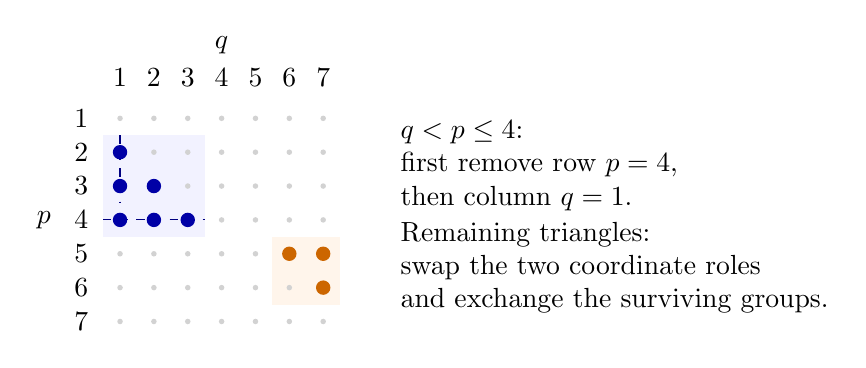
\begin{tikzpicture}[x=.43cm,y=-.43cm]
  \fill[blue!5] (.5,1.5) rectangle (3.5,4.5);
  \fill[orange!8] (5.5,4.5) rectangle (7.5,6.5);
  \draw[blue!50!black,dashed] (.5,4)--(3.5,4);
  \draw[blue!50!black,dashed] (1,1.5)--(1,3.5);
  \foreach \p in {1,...,7}{
    \node[left] at (.35,\p) {$\p$};
    \node[above] at (\p,.35) {$\p$};
    \foreach \q in {1,...,7}{
      \fill[gray!35] (\q,\p) circle (1.0pt);
    }
  }
  \foreach \p/\q in {2/1,3/1,3/2,4/1,4/2,4/3}
    \fill[blue!65!black] (\q,\p) circle (2.6pt);
  \foreach \p/\q in {5/6,5/7,6/7}
    \fill[orange!80!black] (\q,\p) circle (2.6pt);
  \node at (-1.25,4) {$p$};
  \node at (4,-1.15) {$q$};
  \node[anchor=west,align=left] at (9,2.4)
    {$q<p\le4$:\\first remove row $p=4$,\\then column $q=1$.};
  \node[anchor=west,align=left] at (9,5.4)
    {Remaining triangles:\\swap the two coordinate roles\\and exchange the surviving groups.};
\end{tikzpicture}
\caption{The evaluation pattern $Q_s$ for $s=3$, with $n=7$ and $s^2=9$
selected pairs. Removing row $p=s+1$ and then column $q=1$
leaves the pattern for $s-1$ after swapping coordinates and
relabeling the two groups. The gray points are unselected pairs.}
\label{fig:triangular-grid}
\end{figure}


\begin{proof}
The polynomial space has dimension $s^2$, and
\[
  |Q_s|=\frac{s(s+1)}2+\frac{s(s-1)}2=s^2.
\]
It therefore suffices to show that a polynomial $P(u,v)$ of degree at
most $s-1$ in each variable, vanishing at all these points, is zero.
We prove this by induction on $s$.  For $s=1$, $P$ is constant and
vanishes at the single point indexed by $(2,1)$.

Let $s>1$.  The first triangle contains the $s$ points
$(x_{s+1},x_q)$ for $1\leq q\leq s$.  The polynomial
$P(x_{s+1},v)$ has degree at most $s-1$ and $s$ distinct roots, so it
vanishes identically.  Division in the variable $u$ gives
\[
  P(u,v)=(u-x_{s+1})P_1(u,v),
  \qquad \deg_u P_1\leq s-2,\quad\deg_v P_1\leq s-1.
\]
For $p=2,\ldots,s$, the remaining points $(x_p,x_1)$ give
$P_1(x_p,x_1)=0$, since $x_p\ne x_{s+1}$.  Thus
$P_1(u,x_1)$, of degree at most $s-2$, has $s-1$ distinct roots and
vanishes identically.  Factoring in the second variable, we obtain
\begin{equation}
\label{eq:triangle-factorization}
  P(u,v)=(u-x_{s+1})(v-x_1)R(u,v),
  \qquad \deg_u R,\deg_v R\leq s-2.
\end{equation}
At every point in the two remaining triangles the displayed factors
are nonzero.  Hence
\[
  R(x_p,x_q)=0
  \quad\text{if }2\leq q<p\leq s
  \quad\text{or if }s+2\leq p<q\leq2s+1.
\]
Define a tuple of $2s-1$ distinct nodes and a polynomial by
\[
  (y_1,\ldots,y_{2s-1})
   =(x_{s+2},\ldots,x_{2s+1},x_2,\ldots,x_s),
  \qquad S(u,v)=R(v,u).
\]
The lower triangle $q<p\leq s$ for the $y$-tuple becomes the remaining
upper triangle for the $x$-tuple after the coordinate swap.  The upper
triangle $s<p<q\leq2s-1$ becomes the remaining lower triangle.
Consequently $S$ vanishes at every point of the pattern $Q_{s-1}$ for
the $y$-tuple.  The induction hypothesis gives $S=0$, hence $R=0$ and
$P=0$.  This proves injectivity of the square evaluation map and thus
both assertions.
\end{proof}

\begin{lemma}[Rank detector]
\label{lem:detector}
Fix any pairwise distinct real numbers $x_1,\ldots,x_n$, where
$n=2s+1$ and $d=s^2$.  There is a linear map
$\Phi:\R^{n\times n}\longrightarrow\R^{d\times d}$ with the following
properties.
\begin{enumerate}[label=\textup{(\roman*)}]
\item $\Phi$ annihilates every additive matrix
$H(p,q)=r_p+c_q$ and every diagonal matrix.
\item For the coordinate matrix $E_{pq}$, the matrix $\Phi(E_{pq})$
has rank one if $p\ne q$, and is zero if $p=q$.
\item For every strict linear order $\prec$ on $\{1,\ldots,n\}$, the
matrix $\Phi(S_\prec)$ is invertible, where
\[
  S_\prec(p,q)=
  \begin{cases}
    \tfrac12,&p\prec q,\\
    -\tfrac12,&q\prec p,\\
    0,&p=q.
  \end{cases}
\]
\end{enumerate}
The same map has these properties for all orders simultaneously.
\end{lemma}

\begin{proof}
Set
\begin{equation}
\label{eq:detector-definition}
\begin{gathered}
  F(t)=\prod_{p=1}^{n}(t-x_p),\qquad
  h_{pq}=(x_p^a x_q^b)_{0\leq a,b<s},\\
  B_{pq}=\frac{x_p-x_q}{F'(x_p)F'(x_q)}
              h_{pq}h_{pq}^{\mathsf T},\qquad
  \Phi(H)=\sum_{p,q=1}^{n}H(p,q)B_{pq}.
\end{gathered}
\end{equation}
The factors $1/F'(x_p)$ are the classical barycentric weights for Lagrange
interpolation~\cite[Section~3, equation~(3.2)]{BerrutTrefethen2004}.
All denominators are nonzero because the nodes are distinct.
The constant coordinate of $h_{pq}$ is $1$, so $B_{pq}$ has rank one
when $p\ne q$, while $B_{pp}=0$.  This proves \textup{(ii)} and the
annihilation of diagonal matrices.  Rank subadditivity also gives
\begin{equation}
\label{eq:detector-support-bound}
  \rank\Phi(H)\leq
  \bigl|\{(p,q):p\ne q,\ H(p,q)\ne0\}\bigr|.
\end{equation}

For the additive matrices, we use the elementary identity
\begin{equation}
\label{eq:lagrange-vanishing}
  \sum_{p=1}^{n}\frac{A(x_p)}{F'(x_p)}=0
  \qquad\text{if }\deg A\leq n-2.
\end{equation}
Indeed, the polynomials
$F(t)/((t-x_p)F'(x_p))$ have degree $n-1$ and take the coordinate
values $1$ at $x_p$ and $0$ at every other node.  Subtracting their
linear combination with coefficients $A(x_p)$ from $A$ gives a
polynomial of degree at most $n-1$ with $n$ distinct roots, so
\[
  A(t)=\sum_{p=1}^{n}
        A(x_p)\frac{F(t)}{(t-x_p)F'(x_p)}.
\]
Comparison of the coefficients of $t^{n-1}$ proves
\eqref{eq:lagrange-vanishing}.

The entry of $B_{pq}$ indexed by $(a,b)$ and $(a',b')$ is
\[
  \frac{(x_p-x_q)x_p^{a+a'}x_q^{b+b'}}
       {F'(x_p)F'(x_q)}.
\]
Its numerator has degree at most $2s-1=n-2$ in either variable
separately.  Applying \eqref{eq:lagrange-vanishing} with the other
variable fixed proves
\[
  \sum_{q=1}^{n}B_{pq}=0\quad\text{for every }p,
  \qquad
  \sum_{p=1}^{n}B_{pq}=0\quad\text{for every }q.
\]
It follows that $\Phi((r_p+c_q)_{p,q})=0$, completing \textup{(i)}.

It remains to prove \textup{(iii)}.  First take the natural order and
write $S=S_\prec$.  Let $H(p,q)=\mathbf{1}_{q<p}$ and let $\mathbf1$
denote the all-ones column vector.  Then
\[
  S=\tfrac12\mathbf1\mathbf1^{\mathsf T}-H-\tfrac12I_n,
  \qquad \Phi(S)=-\Phi(H).
\]
Subtract $1$ from each row of $H$ indexed by $p>s+1$, obtaining
$H'$.  The difference $H-H'$ is additive, so $\Phi(H')=\Phi(H)$.
Apart from diagonal entries, which $\Phi$ annihilates, the support
of $H'$ is exactly $Q_s$: its value is $+1$ on the first triangle
of \eqref{eq:triangular-pattern} and $-1$ on the second.

List the pairs in $Q_s$ in any order, and let $A_Q$ be the square
matrix with columns $h_{pq}$ in that order.  By
Lemma~\ref{lem:triangular-basis}, $A_Q$ is invertible.  Equation
\eqref{eq:detector-definition} now gives
\begin{equation}
\label{eq:detector-factorization}
  \Phi(S)=-A_Q D_Q A_Q^{\mathsf T},\qquad
  D_Q=\diag\left(
       H'(p,q)\frac{x_p-x_q}{F'(x_p)F'(x_q)}
       \right)_{(p,q)\in Q_s}.
\end{equation}
Every diagonal entry of $D_Q$ is nonzero, so $\Phi(S)$ is invertible.

Finally let $\pi(1)\prec\cdots\prec\pi(n)$ be an arbitrary order.
Relabel the indices and use the tuple
$(x_{\pi(1)},\ldots,x_{\pi(n)})$ in the argument just given.
The relabeled evaluation vector at $(r,q)$ is
$h_{\pi(r),\pi(q)}$, so this only reindexes the sum defining
$\Phi(S_\prec)$; the polynomial $F$ and the fixed map $\Phi$ are
unchanged.  The relabeled nodes are
distinct, so Lemma~\ref{lem:triangular-basis} applies again.
Thus every order has invertible image under the original map.
\end{proof}

\section{The crossing-number formula}
\label{sec:formula}

We now combine the preceding results to prove Theorem~\ref{thm:main}.

\subsection{The upper bound}
We recall the classical axis construction; see
Woodall~\cite[p.~658]{Woodall1993}.
Place the vertices $a_i$ on the vertical axis, divided as evenly as
possible between its positive and negative rays. Place the vertices $b_p$
on the horizontal axis in the same way, and join every required pair by
a straight segment. All positions are distinct and nonzero.
An edge interior is contained in one open quadrant.

In a quadrant whose bounding rays contain $u$ first-class and $v$
second-class vertices, each choice of two vertices on each ray forms a
convex quadrilateral. Exactly its diagonals cross, so the contribution is
$\binom u2\binom v2$.
Summing over the quadrants and using \eqref{eq:dr} gives exactly
$d_m d_n$ crossings, provided no three segments concur in their interiors.

The positions can be chosen to ensure this condition. Three segments
concurrent in their interiors must have six distinct endpoints, since
segments with a common endpoint do not cross elsewhere. Their concurrence
is a proper polynomial condition on their axis intercepts: keeping two
segments fixed and varying an intercept of the third avoids their
intersection. There are only finitely many triples, and the product of
their nonzero defining polynomials cannot vanish on the open set of
permitted positions. Thus an admissible drawing achieves the stated count.
In particular,
\begin{equation}
\label{eq:upper}
 \crn(K_{m,n})\le d_m d_n.
\end{equation}
If $m\le2$ or $n\le2$, this already proves equality by nonnegativity.

\subsection{The lower bound for odd \texorpdfstring{$n$}{n}}
Assume $m\ge3$ and $n=2s+1\ge3$, and put $d=s^2=d_n$.
Choose a minimum drawing $D$ normalized as in
Lemma~\ref{lem:normalization}. In particular, no two edges with a common
endpoint cross. Form the blocks $J^{ik}$ of its signed-intersection matrix.
Use the map $\Phi$ from Lemma~\ref{lem:detector}, with any one tuple of
distinct nodes, and set
\[
 R_{ik}=\Phi(J^{ik}),\qquad
 X_i=R_{i1},\qquad Y_k=R_{11}-R_{1k}.
\]
Lemma~\ref{lem:additive} and the annihilation property of $\Phi$ imply
\begin{equation}
\label{eq:rank-family}
 R_{ik}=X_i-Y_k.
\end{equation}
Thus the matrices have the difference form required by
Corollary~\ref{cor:rank-sum}.  We next check its invertibility hypothesis
on diagonal blocks and bound the other block ranks by crossings.

All edges in the star at $a_i$ are oriented outward and do not cross one
another. Consequently $J^{ii}$ is exactly half the sign matrix of the
linear spoke order at $a_i$. Lemma~\ref{lem:detector} gives
\begin{equation}
\label{eq:diagonal-ranks}
 \rank R_{ii}=d\qquad(1\le i\le m).
\end{equation}

For $i\ne k$, let $c_{ik}$ be the number of crossing points between
edges incident with $a_i$ and edges incident with $a_k$.
The entries $J^{ik}(p,p)$ may contain a local term at $b_p$, but $\Phi$
annihilates all diagonal entries: the factor $x_p-x_q$ in
\eqref{eq:detector-definition} makes $B_{pp}=0$.
If $p\ne q$, the two edges $ip,kq$
have no common endpoint, so $J^{ik}(p,q)=I(ip,kq)$.
Each nonzero such entry requires at least one crossing and contributes
to $R_{ik}$ a matrix of rank at most one. Rank subadditivity yields
\begin{equation}
\label{eq:crossing-rank}
 \rank R_{ik}\le c_{ik}\qquad(i\ne k).
\end{equation}
This estimate counts crossing points correctly even when a pair of
edges crosses repeatedly: cancellation in the signed sum can only reduce
the number of nonzero contributions.

Corollary~\ref{cor:rank-sum}, applied to
\eqref{eq:rank-family}--\eqref{eq:diagonal-ranks}, now gives
\[
 2d_m d
 \le \sum_{i\ne k}\rank R_{ik}
 \le \sum_{i\ne k}c_{ik}
 =2c(D).
\]
The last equality holds because each crossing belongs to exactly two
ordered pairs of distinct first-class stars.
Thus $\crn(K_{m,n})\ge d_m d_n$ for odd $n\ge3$.

\subsection{The even case}
We use the vertex-deletion count appearing in
Kleitman~\cite[Section~3, equations~(6)--(7)]{Kleitman1970} and
Woodall~\cite[Theorem~1 and Corollary~1.1]{Woodall1993}.
Let $n>2$ be even, and start again with a normalized minimum drawing $D$.
Delete each of its $n$ second-class vertices in turn. Each remaining
$K_{m,n-1}$ drawing has at least $d_m d_{n-1}$ crossings by the odd case.
Since the two edges at any crossing have distinct second-class endpoints,
that crossing remains in exactly $n-2$ of the deleted-vertex drawings.
Therefore
\[
 (n-2)c(D)\ge n d_m d_{n-1}=(n-2)d_m d_n,
\]
where the last identity follows directly from \eqref{eq:dr} for even $n$.
Division by $n-2$ and the upper bound \eqref{eq:upper} prove equality.
Together with the zero-factor cases, this completes
Theorem~\ref{thm:main}. \qed


\appendix
\section{Normalization of continuous-arc drawings}
\label{sec:normalization}

This appendix supplies the drawing reduction used in
Section~\ref{sec:intersections}.  The argument applies to any finite
simple graph and counts every crossing point separately. The removal
of adjacent-edge crossings is a standard ordinary-crossing reduction
\cite{FulekEtAl2012}; we include the continuous-arc details.

\begin{lemma}[Drawing normalization]
\label{lem:normalization}
An admissible continuous-arc drawing of a finite simple graph can be
replaced by a polygonal drawing with no more crossing points, with
edges straight near every vertex and crossing, and with no crossings
between edges sharing an endpoint.  In particular, a drawing attaining
the ordinary crossing number can be chosen to have these properties.
\end{lemma}

\begin{proof}
\emph{Isolating the marked passages.}
Call the vertices and crossing points of the given drawing its
\emph{marks}.  There are finitely many.  Parameterize each edge
injectively by $\gamma_e:[0,1]\to\R^2$.  On each edge, choose pairwise
disjoint parameter neighborhoods of its marked parameters, with
disjoint closures, using one-sided neighborhoods at $0$ and $1$.
For a mark $w$ on that edge, the image of the compact parameter set
outside its chosen neighborhood avoids $w$, and hence has positive
distance from $w$.  If $w$ is not on the edge, the entire compact edge
image has positive distance from $w$.  Since all these conditions are
finite, we may choose pairwise disjoint closed round disks $D_w$,
centered at the marks, so that every visit of an edge to $D_w$ is in
its prescribed parameter neighborhood, and nonincident edges avoid
$D_w$ altogether.

For an interior mark on $e$, remove the parameter interval from the
first to the last visit to $D_w$.  This removes the intervening
excursions too.  At the starting endpoint remove the interval through
the last visit to its disk; at the terminal endpoint remove the
interval from the first visit to its disk.  These removed intervals
are disjoint along each edge.  The retained middle pieces are compact
arcs with endpoints on disk boundaries and interiors in
\[
 \Omega=\R^2\setminus\bigcup_w D_w.
\]
They are pairwise disjoint, with distinct endpoints: every possible
intersection in the original drawing was a mark and has been removed.
This construction uses the first and last visits to each \emph{closed}
disk, which exist by compactness.  It does not require an arc to cross
a round disk boundary only finitely many times.

\emph{Replacing the exterior pieces.}
The finitely many disjoint compact middle pieces admit pairwise
disjoint open neighborhoods $U_P$.  For a boundary endpoint $x$ of
one piece $P$, take a short straight spur from $x$ radially outward
from its disk.  Its interior lies in $U_P\cap\Omega$.
The spur tip can be connected to a nearby interior point of $P$ in
that same open set.  To see this directly, a sufficiently small
exterior collar at $x$ lies in $U_P$ and meets no other disk.  In polar
coordinates about the disk center, choose the collar to have radius
in $(r,r+\delta)$ and angle in a small open interval about the angle
of $x$, where $r$ is the disk radius.  It contains both the spur tip
and all sufficiently nearby interior points of $P$.  Radial paths
and a short concentric arc connect those points inside the collar.
Do this at both ends of $P$ and use the original middle subarc between
the selected interior points.  The resulting connection between the
two spur tips lies in $U_P\cap\Omega$.

Any continuous path with compact image in an open subset of the plane
can be replaced, with the same endpoints, by a polygonal path in that
open set: cover its image by small balls in the set, subdivide its
parameter interval so each subarc lies in one such ball, and join
successive subdivision points by straight segments there.  Apply this
to the connection just obtained, then attach the two spurs.  If the
result has loops, subdivide the finite union of its segments at all
segment endpoints and intersections; for collinear overlaps, also
subdivide at the overlap endpoints and identify coincident pieces.
This is a finite embedded graph.  A simple graph path between the
original boundary endpoints is a simple polygonal arc, still in
$U_P$ with its interior in $\Omega$.  Carry out this construction for
every $P$.  Their disjoint neighborhoods ensure that no resulting
exterior pieces meet.

\emph{Filling the disks.}
In a crossing disk join each of its two pairs of boundary endpoints
by a straight chord.  The four endpoints are distinct.  The chords
can therefore meet at most once, and any meeting is an interior
transverse crossing: a line cannot contain four distinct points of a
circle.  In a vertex disk choose a new vertex point in its interior
off the finitely many lines through pairs of its boundary endpoints,
and join all the endpoints to it by straight spokes.  These spokes
meet only at the vertex.  The new vertex points in different disks
are distinct.

Assemble the spokes, chords, and exterior polygonal pieces in their
original edge order.  Each resulting edge is simple: the exterior
pieces are disjoint, the disks are disjoint, and an edge uses at most
one chord or spoke in any one disk.  Its interior avoids all vertices.
Every inter-edge crossing lies in an original crossing disk, with at
most one crossing in that disk and no third edge there.  Thus the
result is admissible, polygonal, and has no more crossings than the
given drawing.  It is straight near every vertex and every crossing.

\emph{Removing adjacent-edge crossings.}
Suppose two polygonal edges $e=vu$ and $f=vw$ sharing $v$ cross at
$x$.  As the graph is simple, $u\ne w$.  Choose a small round disk
about $x$ that meets only the two straight crossing strands and
contains no other mark or bend.  Swap the portions of $e$ and $f$
from $v$ up to this disk, then connect the swapped prefixes to the
original suffixes.  Inside the disk this pairs adjacent boundary
endpoints, so two disjoint chords make the reconnections.  The result
is a walk from $v$ to $u$ and a walk from $v$ to $w$.  The crossing
at $x$ has disappeared.  Outside the disk every old open track is
assigned exactly once in total to the two new walks.

The walks may have self-intersections.  Subdivide their tracks at
all remaining intersections and bends, and repeatedly delete the
closed subwalk between two occurrences of the same subdivision
vertex.  Each deletion shortens a finite walk, so it yields a simple
polygonal path between the required endpoints.  We check that this
operation preserves admissibility.  At an old crossing of $e$ and
$f$ distinct from $x$, either the two straight-through tracks belong
to different new walks, or both belong to one walk.  In the first
case each walk visits that point only once; loop deletion either
removes its passage or retains its original straight-through
passage.  In the second case loop deletion may create a turn at that
point, but neither the other walk nor a third edge is present there.
Likewise, a crossing with any third edge occurs on a track visited
at most once by the two walks together, and any retained passage is
straight-through.  These observations cover every possible meeting:
the original drawing had no triple crossings and no common subarcs.
The tracks avoid graph vertices in their interiors, and each walk
visits its initial and terminal graph vertices only at its ends.
Hence the simplified paths are admissible edges, with no new
crossing or improper meeting.

The crossing at $x$ has been removed and none has been added.
Repeat this operation while an adjacent-edge crossing remains.  The
nonnegative integer crossing count decreases at every step, so the
process terminates.  Remaining crossings are still locally straight;
any new turn occurs away from all other edges.  The straight spokes
at vertices are merely reassigned among the two incident edges.
Small disjoint vertex, crossing, and bend disks can be chosen afresh
afterwards.  This proves all asserted properties.
\end{proof}


\begingroup
\small
\raggedright
\bibliographystyle{plain}
\bibliography{references}
\endgroup
\end{document}
